統計情報提供機能は,年代,性別の違いから情報倫理に関する意識に違いが生まれていることから\cite{isiki},教材提供者が作成した問題を学習者が解いた際の回答情報を基に,グラフで統計情報を提供する機能である.
これにより,教材提供者は作成したコンテンツの質を向上させることができる.
提示する統計情報の内容としては,問題の各選択肢における割合や回答者の年齢層,性別である.
統計情報提供機能のGUIは図\ref{toukei_ex}の通りである.

\begin{figure}[htbp]
    \begin{center}
        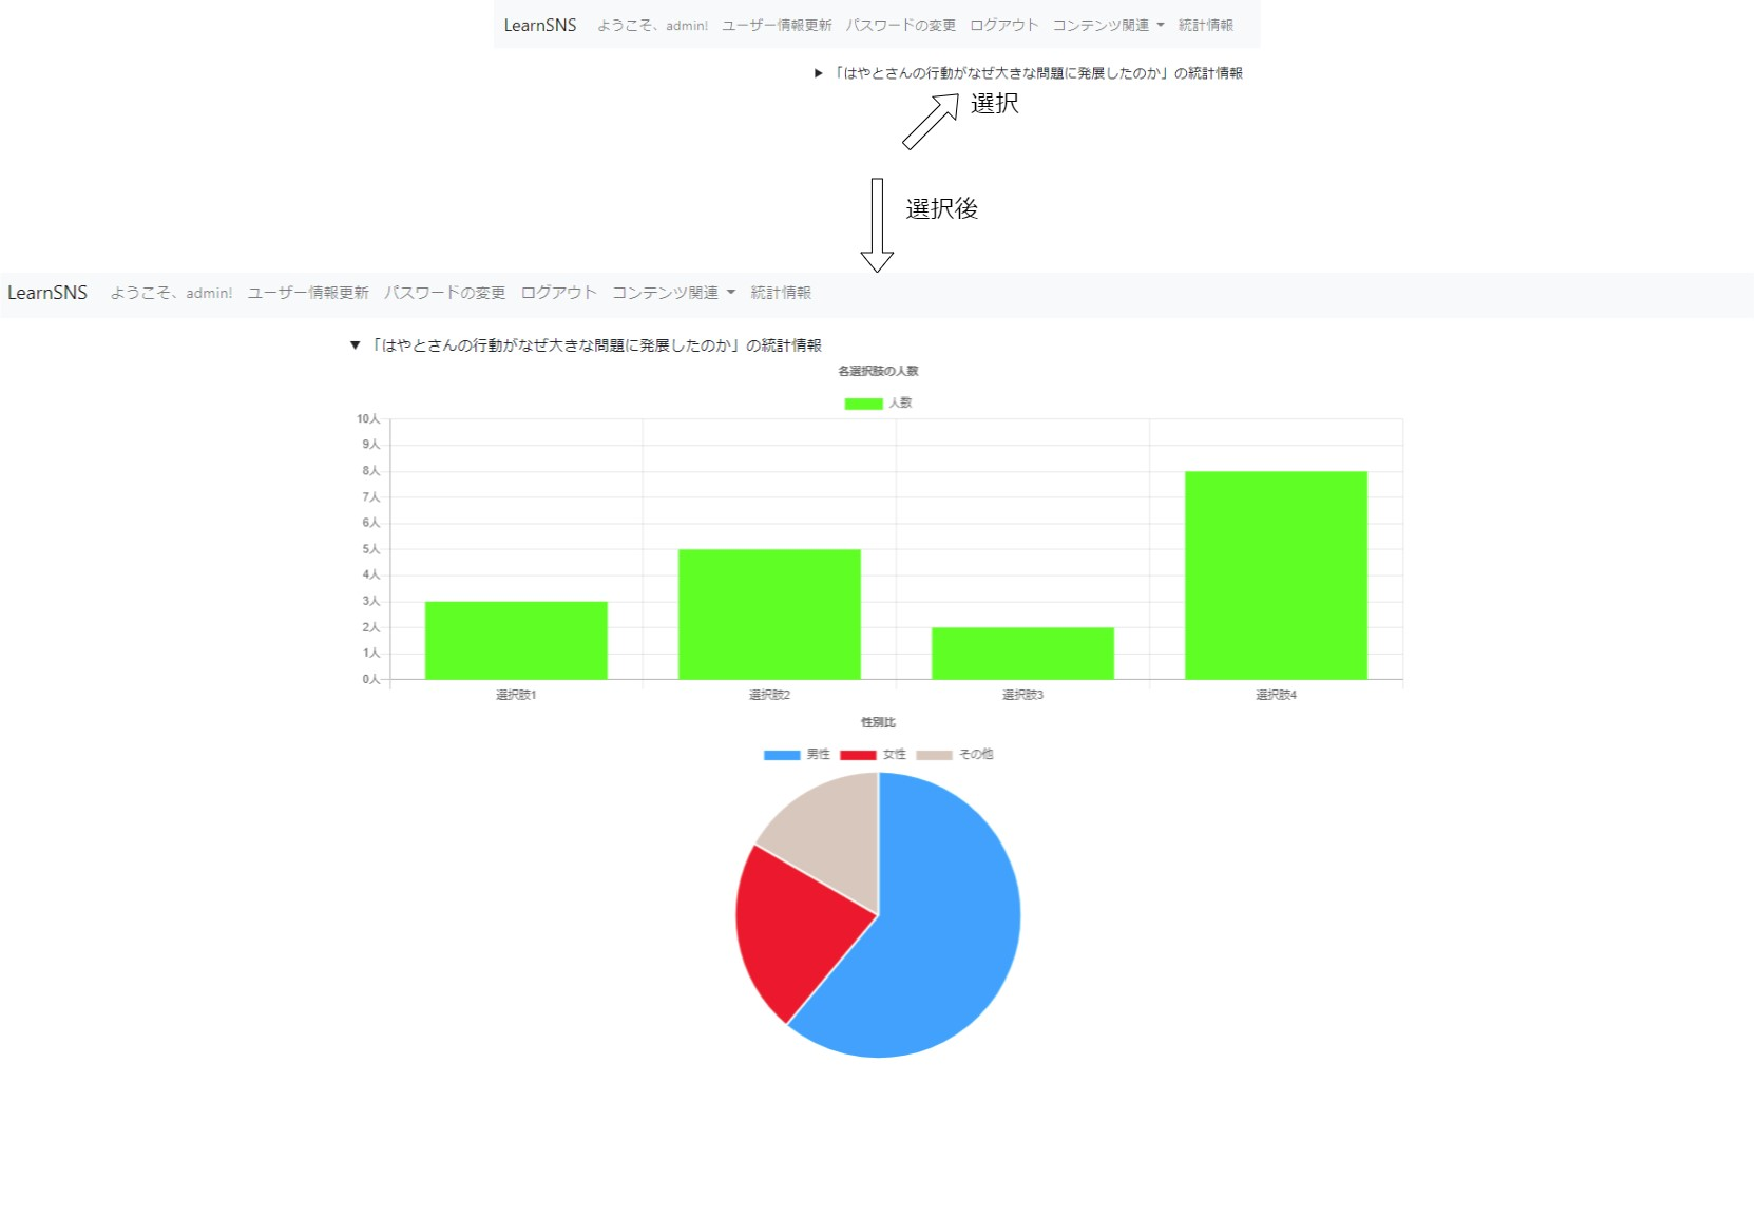
\includegraphics[width=18cm,height=17cm,keepaspectratio]{toukei_ex-crop.pdf}\\
        %includegraphicsの詳しい使い方ははLaTeXの参考書を参照.
    \end{center}
    \caption{統計情報提供機能のGUI}
    \label{toukei_ex}
\end{figure}

\newpage
本機能はChart.jsというjavascriptで作成されたグラフ描画ライブラリを作成している.
Chart.jsでは線グラフ,棒グラフ,レーダーチャート,鶏頭図,ドーナツチャート,円グラフ,バブルチャートを作成できる.
本機能では,棒グラフと円グラフを使用している.

また,本機能で取得可能な情報を表\ref{toukei_info}に示す.
これらの取得できる情報を使って教材提供者はChart.jsで新たなグラフを挿入することができる.

\begin{table}[htb]
    \begin{center}
        \caption{取得可能情報一覧}
            \begin{tabular}{|l|l|} \hline
                取得可能情報 & 詳細 \\ \hline
                学習者情報 &   
                \begin{tabular}{l}
                    年齢\\性別\\回答した問題・選択肢 
                \end{tabular}\\ \hline
                コンテンツ情報 & 問題に対応したコンテンツ \\ \hline
            \end{tabular}
    \label{toukei_info}
    \end{center}
\end{table}